\documentclass{article}
\usepackage{graphicx}
\usepackage{float}
\usepackage{subcaption}
\usepackage{amsmath}
\usepackage[final]{pdfpages}
\usepackage{hyperref}
\usepackage{titlesec}
\usepackage{caption}
\captionsetup[figure]{labelformat=empty}
\hypersetup{
colorlinks,
citecolor=black,
filecolor=black,
linkcolor=black,
urlcolor=black
}
\titlespacing*{\section}{0pt}{1cm}{0.5cm}
\titlespacing*{\subsection}{0pt}{0.5cm}{0.5cm}
\title{Travlendar+ \\Requirement Analysis and Specification Document}
\author{Fumagalli Paolo, Grotti Pietro, Gullo Marco}
\begin{document}
\pagenumbering{roman}


\begin{figure}[t]

\includegraphics[width=\linewidth]{Logo_Politecnico_Milano.png}
\label{fig:Logo}
\end{figure}
\maketitle
\newpage
\tableofcontents
\newpage
\pagenumbering{arabic}
\section{Introduction}
\subsection{Purpose}
\paragraph{}
Many endeavors require scheduling meetings at various locations all across a city, whether in support of a mobile job or a busy parent. The goal of this project is to create a calendar interface that automatically computes and accounts for travel time between appointments to make sure that you're never late for an appointment. The application will also suggest travel means by appointment (e.g., perhaps you drive to the office in the morning but the bus is a better choice between a pair of afternoon meetings) and by day ( e.g. working days or weekends, traffic, public transport strikes, weather). The application will support an user interface where complete and automatically well-fitted schedules can be made. System will alert for any appointment overlap and non-doable consecutive appointments (e.g. two meetings really close in time but in locations too far from each other). Furthermore, different preferences, such as travel options and break time, can be expressed by the user.
\paragraph{Goals\\} The application has the following goals:
\begin{enumerate}
\item[\textbf{G1:}] Allow a guest user to register to Travlendar+ by filling the registration form with the data needed.
\item[\textbf{G2:}] Allow the user to select preferences and modify them whenever he wants.
\item[\textbf{G3:}] Allow the user to easily create an organized and customizable agenda based on his preferences.
\item[\textbf{G4:}] To help the user plan his movements in a clever and efficient way.
\item[\textbf{G5:}] To guarantee the user no to be late for his appointments.
\begin{enumerate}
\item[\textbf{G5.1:}] The system will take into account the possibility of accidents and plan for the user to arrive at least 10 minutes before the beginning of the event.
\item[\textbf{G5.2:}] The user will be notified if an appointment is not reachable in time.
\end{enumerate}
\item[\textbf{G6:}] To let the users buy bus or train tickets (both single or seasonal).
\item[\textbf{G7:}] To let the user find vehicles from vehicle sharing systems.
\item[\textbf{G8:}] Allow the user to buy in advance tickets which can be used later on.
\end{enumerate}
\newpage
\subsection{Scope}
\paragraph{}
Travlendar+ is an application which will be able to manage daily appointments of the users and assist them by creating a specific course around the city which will identify the best mobility option to move from one appointment to the other. It will consider all public transportation options (train, metro, bus, etc.), car and bike sharing systems, the eventuality of a private vehicle and the weather conditions as well, to avoid having the user bike in harsh weather conditions or when it is too hot. It will also be possible to buy tickets and locate cars and bikes directly through the application. Users will have to create meetings specifying the location, the date and the time and the application will automatically calculate the suggested course and travel time, if it is impossible to reach a certain meeting in time the application will send a warning to the user. It will also feature the possibility of selecting a time span in which it will have to save some time for a break in which the user can have lunch (for example if the user wants to have lunch between 11:30 to 2:30 and it should be at least half an hour long, the application will reserve at least 30 minutes for lunch every day). Travlendar+ will also give the possibility to the users to buy tickets, this will make it easier to move with public transportation around the city. To allow these transactions the system will have to work with a bank which will support the possibility of either using a credit/debit card to buy tickets or creating a balance that will be connected to the account. The balance can be charged by credit/debit card or through selected shops which will allow the acquisition of cards containing unique codes, which will load money on the balance.
\subsection{Definitions, Acronyms, Abbreviations}
\subsubsection{Definitions}
\subsubsection{Abbreviations}
G* : Specific goal\\ R* : Specific functional requirements\\ D* : Specific domain assumption \\ App : Application
\subsubsection{Acronyms}
ETA : Estimated Time of Arrival\\ API : Application Programming Interface\\ PTS : Public Transportation System\\ CSS : Car-Sharing System\\ BSS : Bike-Sharing System
\subsection{Revision history}
Version 1.0.0
\subsection{Reference Documents}
\begin{itemize}
\item{} IEEE Recommended Practice for Software Requirements Specifications, Software Engineering Standards Committe, 1998
\item{} Specification Document: “Mandatory Project Assignments 2017-2018”
\item{} \href{https://www.programmableweb.com/api-university/what-are-apis-and-how-do-they-work}{API overall description}
\item{} \href{http://ieeexplore.ieee.org/stamp/stamp.jsp?arnumber=392555}{RASD structure according IEEE standard}
\end{itemize}
\subsection{Document Structure}
We decided to structure the document starting from the IEEE standard, but modifying it to make it more readable and linear.\\ Chapter 2 will give an overall presentation of the application, starting with the purpose of the project and later defining which will be the actors interacting with Travlendar+ and which are the assumptions that we will consider as true for the development of the project.\\ Later in chapter 3 we will define all the requirements, both functional and non-functional. In this chapter we will include some initial mock-ups of the application.\\We've decided to divide the requirements from the diagrams, so chapter 4 will contain all of our UML, Use Cases, Statecharts and Sequence Diagrams, which will be related to the goals and requirements we defined before this chapter.\\ Chapter 5 will show a formal analysis of the application which was created in Alloy, and it will also show some instances of the application.
\newpage
\section{Overall Description}
\subsection{Product perspective}
\begin{figure}[H]
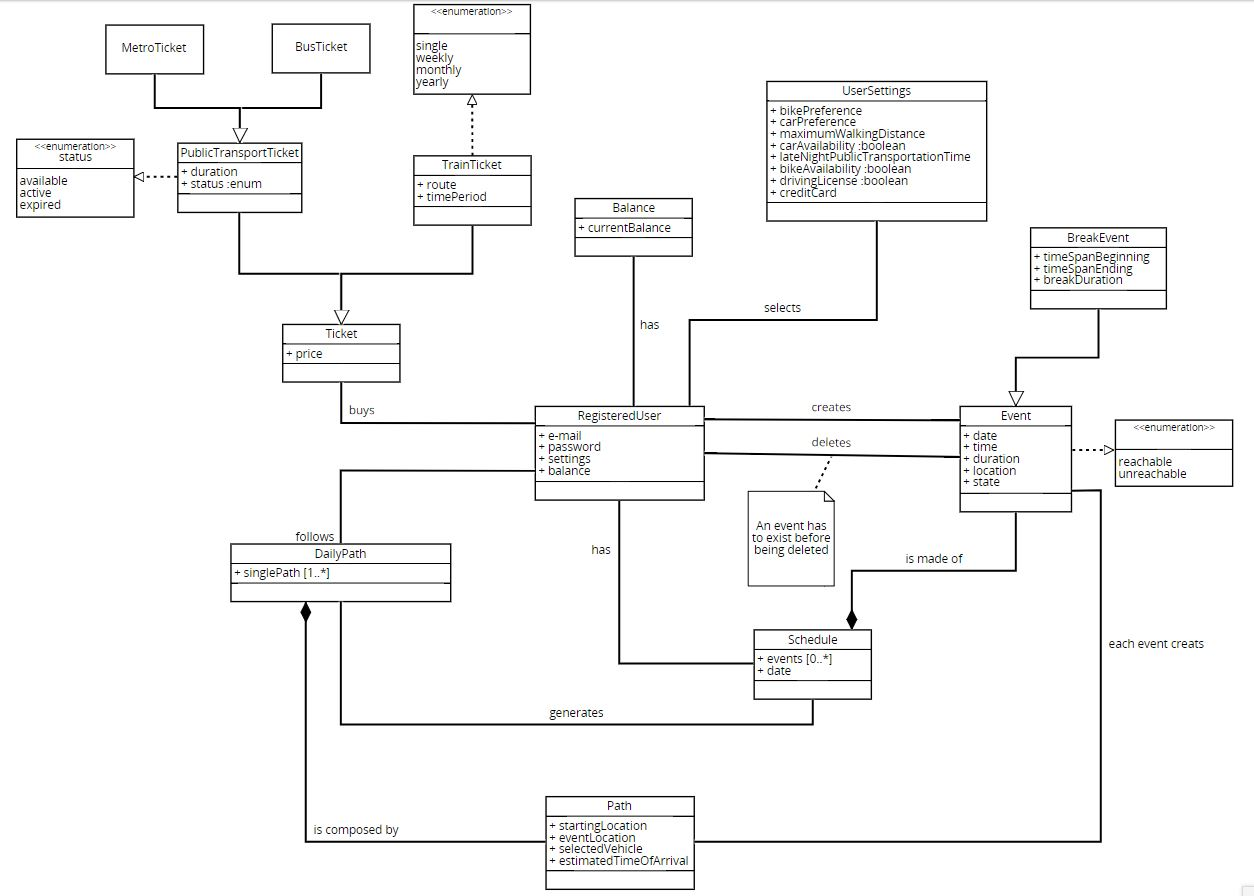
\includegraphics[width=\linewidth]{Class_Diagram}
\caption{Class Diagram}
\label{fig:CD}
\end{figure}

The product’s main purpose is to fit in user’s everyday reality, dealing with a large number of external factors and environments, such as weather conditions, traffic, news, etc. In order to face up all these agents, the system will always cooperate with other existing applications and ask for external help. Travlendar+ will work as an agent-in-the-middle between user and different interfaces, putting together all data required for user’s planning and traveling needs. All the various interactions will be described in high-level details in UML Section (see Section 4.2: Use Cases). 
\subsection{Product functions}
All main functions will be described in following sections (see Section 3: Specific Requirements) and are the ones that will cover all project goals provided above(see Section 1.1: Purpose). 
\subsection{User characteristics}
\paragraph{Actors:}
\begin{itemize}
\item \textbf{Guest User:} unregistered customer, he has just downloaded the app or visited the website. He wants to try Travlendar+ and needs to find a user-friendly interface.
\item \textbf{Registered User:} more familiar with the environment, can access all Travlendar+ functionalities and customize his preferences. Expects an efficient service.
\item \textbf{Public Transportation System:} local public transportation business, is willing to cooperate with the app in order to increase tickets’ sales and reduce irregular PTS use. Online purchases may also decrease the costs of printed tickets. 
\item \textbf{Car-sharing System:} local private enterprise, is interested in Travlendar+ development to enhance their business’ reach and visibility. 
\item \textbf{Bike-sharing System:} same as car-sharing system.
\item \textbf{Google Maps:} is a web mapping service developed by Google. It offers satellite imagery, street maps, 360° panoramic views of streets, real-time traffic conditions, and route planning for traveling by foot, car or public transportation. It is completely free-to-use (its API can be integrated easily in any system) for any system. Travlendar+ will benefit of this.
\item \textbf{Bank:} it is the entity necessary for Travlendar+ to deal with money transactions (ticket and pass purchases). The bank surely has its own secure channels and count on integrity of data coming from the app’s system.
\end{itemize}
\subsection{Assumptions, dependencies and constraints}
The following assumptions are to be considered true in the world that we will analyize:
\begin{enumerate}
\item[\textbf{D1:}] The city is covered by several public and private transport services.
\item[\textbf{D2:}] The services are almost always available, and when they aren’t there’s an alternative which can be suggested by Travlendar+ to the user.
\item[\textbf{D3:}] A database containing all the correct information needed for transport services (location of the vehicles or the stationts, time tables, etc.) is connected to Travlendar+.
\item[\textbf{D4:}] An application able to calculate travel times and distances which can also access current traffic information is connected to Travlendar+.
\item[\textbf{D5:}] Some services allow external applications to interact with them to take advantage of certain functions (e.g.: to buy bus tickets from the PTS or to find a car of a BSS) in a transparent way from the user's point of view.
\item[\textbf{D6.}] An internet connection is available everywhere and at any given time in the area covered by Travlendar+.
\item[\textbf{D7:}] Users of the application have a working GPS that can accurately calculate their position.
\item[\textbf{D8:}] The public transportation companies agree to let the application developers sell tickets through Travlendar+.
\item[\textbf{D9:}] The transactions are handled through a bank that agrees to work with Travlendar+.
\item[\textbf{D10:}] Bikes and cars of sharing-systems are equipped with an accurate GPS that can be traced in the map.
\item[\textbf{D11:}] Vehicles sharing systems agree to work with Travlendar+.
\item[\textbf{D12:}] "Activated" tickets are accepted by public transportation companies.
\end{enumerate}
\newpage
\section{Specific Requirements}

\subsection{External Interface Requirements}
\subsubsection{User Interfaces}
\paragraph{}
In the following section we will show some mock-ups of how the application will look like from the user's point of view.
\begin{figure}[H]
\minipage{0.32\textwidth}
  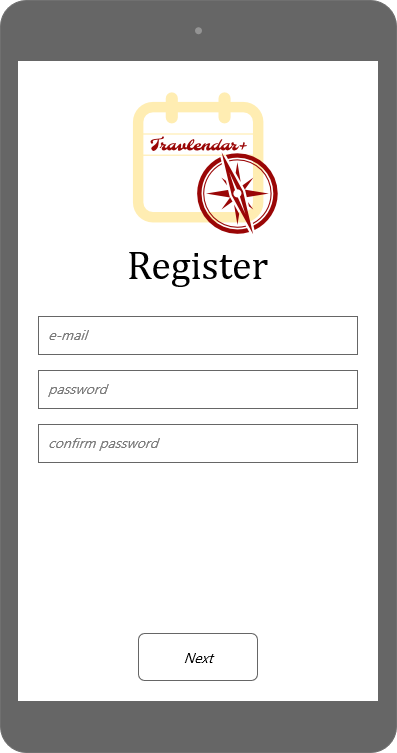
\includegraphics[width=\linewidth]{01-email_and_password.png}
  \caption{Account Creation}\label{fig:MU1}
\endminipage\hfill
\minipage{0.32\textwidth}
  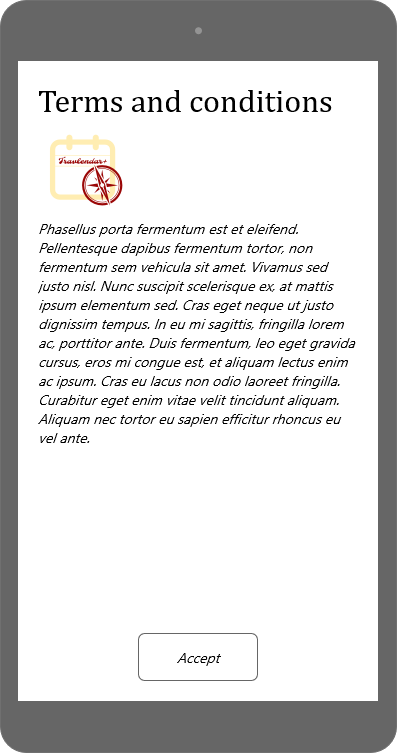
\includegraphics[width=\linewidth]{02-Terms_and_conditions.png}
  \caption{Terms And Conditions}\label{fig:MU2}
\endminipage\hfill
\minipage{0.32\textwidth}
  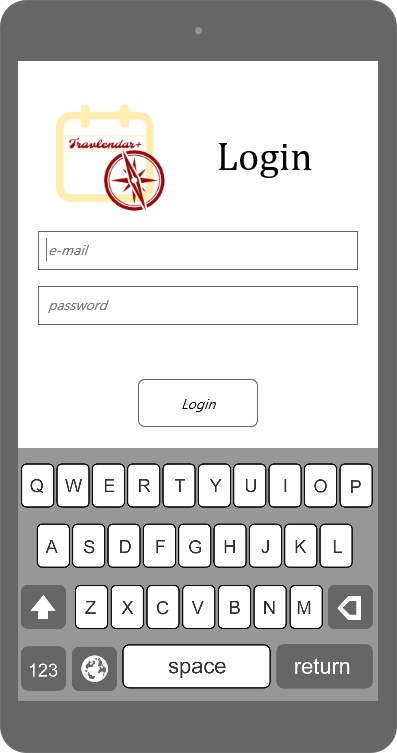
\includegraphics[width=\linewidth]{03-login.png}
  \caption{Login}\label{fig:MU3}
\endminipage
\end{figure}
\begin{figure}[H]
\minipage{0.32\textwidth}
  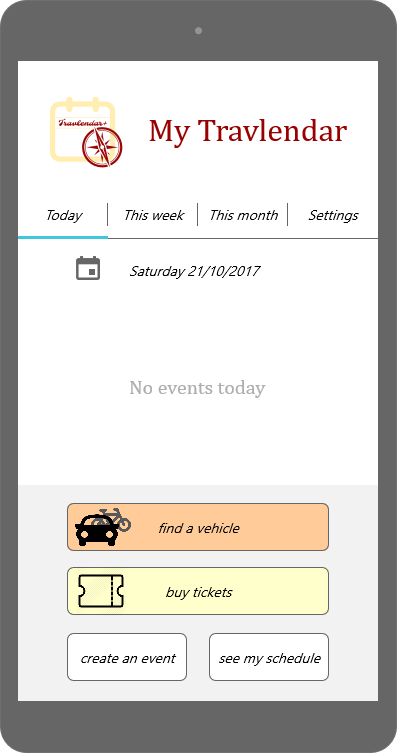
\includegraphics[width=\linewidth]{01-Home_Page.png}
  \caption{Home Page}\label{fig:MU4}
\endminipage\hfill
\minipage{0.32\textwidth}
  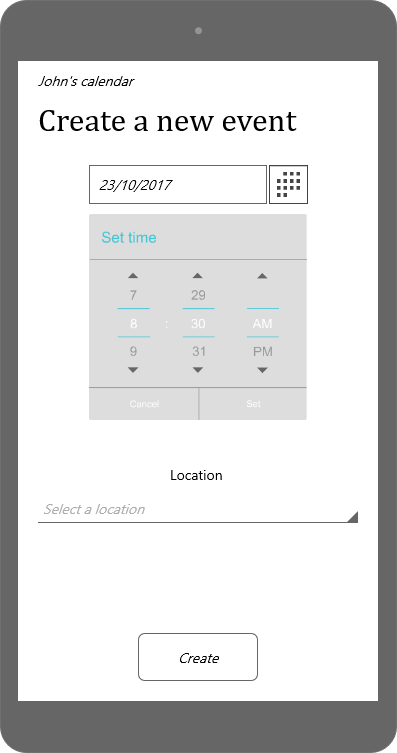
\includegraphics[width=\linewidth]{02-Create_an_event.png}
  \caption{Create Event}\label{fig:MU5}
\endminipage\hfill
\minipage{0.32\textwidth}
  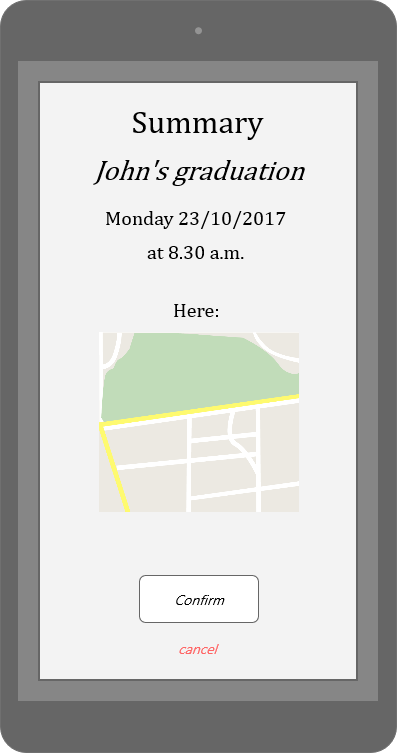
\includegraphics[width=\linewidth]{03-Summary.png}
  \caption{Summary}\label{fig:MU6}
\endminipage
\end{figure}
\begin{figure}[H]
\minipage{0.32\textwidth}
  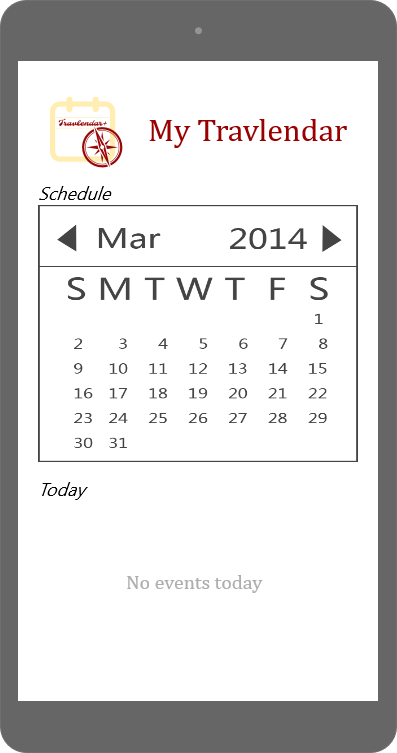
\includegraphics[width=\linewidth]{04-Schedule.png}
  \caption{Schedule}\label{fig:MU7}
\endminipage\hfill
\minipage{0.32\textwidth}
  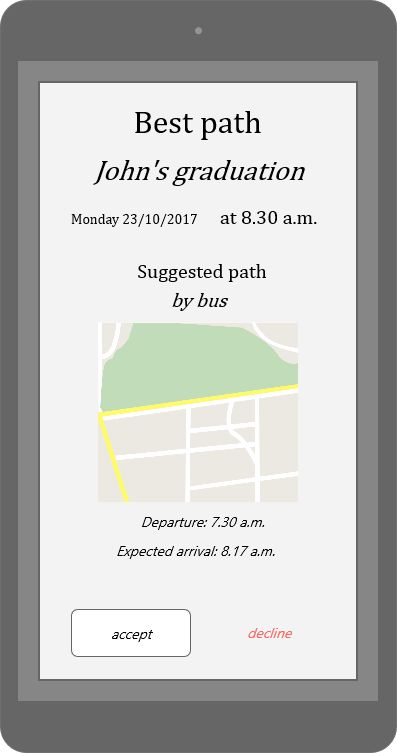
\includegraphics[width=\linewidth]{05-Path.png}
  \caption{Path}\label{fig:MU8}
\endminipage\hfill
\minipage{0.32\textwidth}
  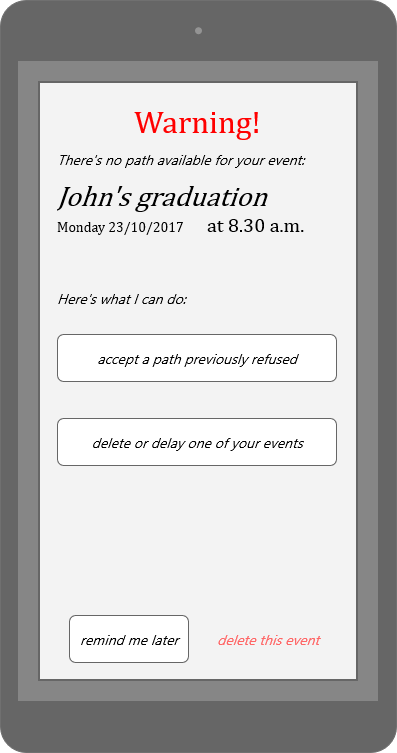
\includegraphics[width=\linewidth]{06-Path_not_available.png}
  \caption{Unreachable Path}\label{fig:MU9}
\endminipage
\end{figure}
\begin{figure}[H]
\minipage{0.32\textwidth}
  \includegraphics[width=\linewidth]{01-Ticket_Store.png}
  \caption{Ticket Store}\label{fig:MU10}
\endminipage\hfill
\minipage{0.32\textwidth}
  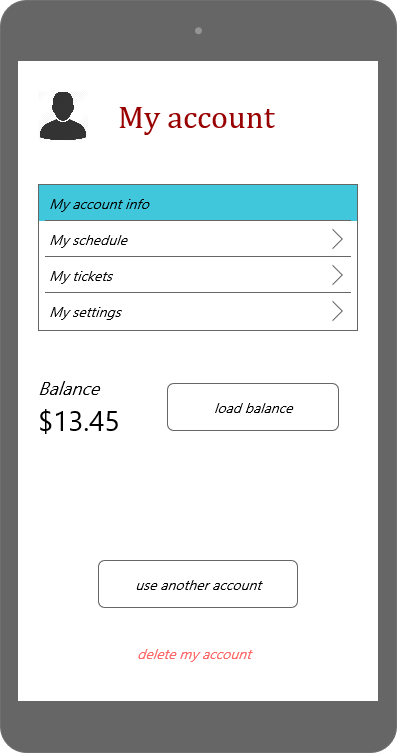
\includegraphics[width=\linewidth]{02-Personal_page.png}
  \caption{Personal Page}\label{fig:MU11}
\endminipage\hfill
\minipage{0.32\textwidth}
  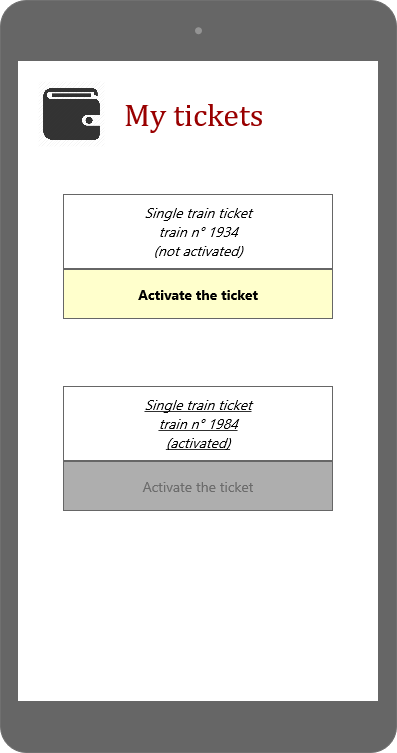
\includegraphics[width=\linewidth]{03-Ticket_Wallet.png}
  \caption{My Tickets}\label{fig:MU12}
\endminipage
\end{figure}
\begin{figure}[H]
\minipage{0.32\textwidth}
  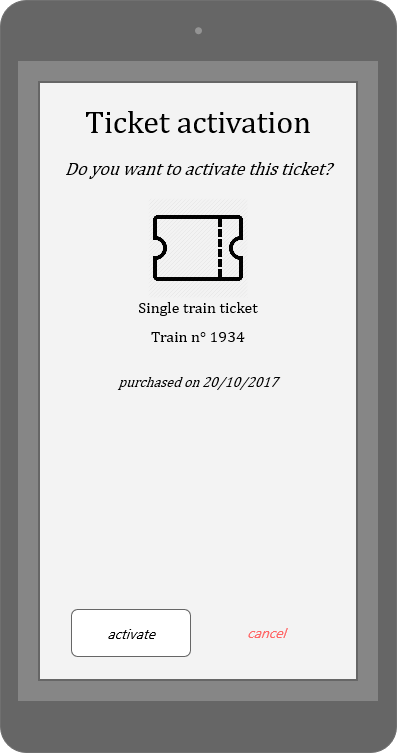
\includegraphics[width=\linewidth]{04-Ticket_activation.png}
  \caption{Ticket Activation}\label{fig:MU13}
\endminipage\hfill
\minipage{0.32\textwidth}
  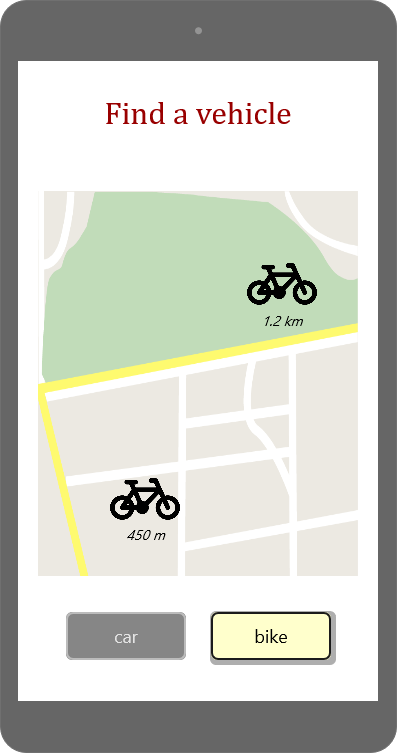
\includegraphics[width=\linewidth]{05-Find_a_vehicle.png}
  \caption{Find a Vehicle}\label{fig:MU14}
\endminipage\hfill
\minipage{0.32\textwidth}
  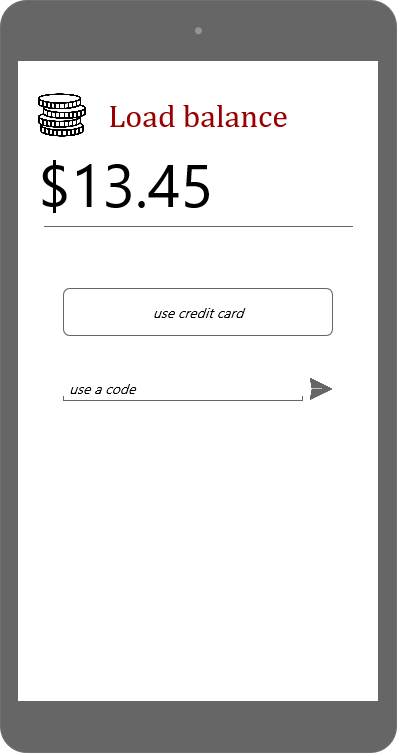
\includegraphics[width=\linewidth]{06-Balance.png}
  \caption{Balance}\label{fig:MU15}
\endminipage
\end{figure}
\begin{figure}[H]
\centering
\minipage{0.32\textwidth}
  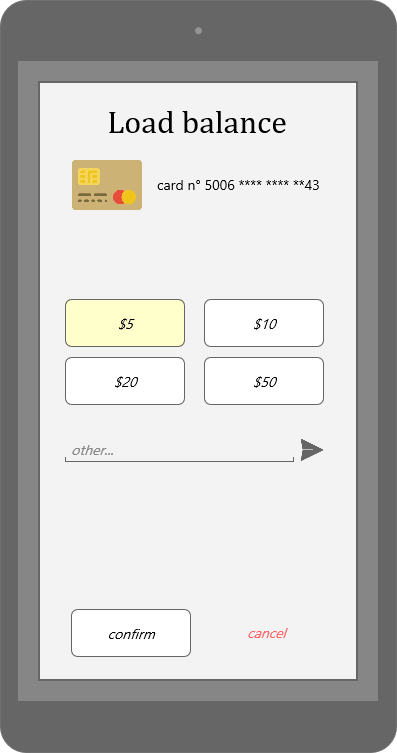
\includegraphics[width=\linewidth]{07-Credit_card_balance_loading.png}
  \caption{Balance Loading}\label{fig:MU16}
\endminipage\hfill
\end{figure}
\newpage
\subsection{Functional Requirements}
In this section we will define the functional requirements combined with the domain assumptions that are needed to reach the goals set in the Section 1.1.
\begin{enumerate}
\item[\textbf{G1:}] Allow a guest user to register to Travlendar+ by filling the registration form with the data needed.
\begin{enumerate}
\item[\textbf{R1:}] A guest user can create a new account through the registration process by providing his credentials to the system. An e-mail will be necessary and it must be unique.
\item[\textbf{R2:}] At the end of the registration process the system will send an e-mail to the user to verify the account.
\item[\textbf{R3:}] The account must be verified with the link provided by the system before it becomes active.
\item[\textbf{R4:}] A guest user can log in the application with his credentials.
\end{enumerate}
\item[\textbf{G2:}] Allow the user to select preferences and modify them whenever he wants.
\begin{enumerate}
\item[\textbf{R5:}] A registered user can modify his preferences by choosing the preferred movement system at any time.
\item[\textbf{R6:}] A registered user can select a specific time during the day (or night) after which he doesn't want to take public transportation.
\item[\textbf{R7:}] A registered user can choose a maximum distance that he is willing to walk to move from one place to the other.
\end{enumerate}
\item[\textbf{G3:}] Allow the user to easily create an organized and customizable agenda based on his preferences.
\begin{enumerate}
\item[\textbf{R8:}] A registered user can create an event by filling the time, date, duration and location of the event.
\item[\textbf{R9:}] A registered user can select a time slot during the day in which he wants to take a break, he can also choose the length of the break (which doesn't have to necessarily be equal to the time slot).
\end{enumerate}
\item[\textbf{G4:}] To help the user plan his movements in a clever and efficient way.
\begin{enumerate}
\item[\textbf{R10:}] The user has to declare if he has a driving license.
\item[\textbf{R11:}] The user can declare if he owns a personal vehicle and indicate which kind of vehicle (car, motorbike, bike).
\item[\textbf{R12:}] The system has to calculate a route to move araound the city based on the user's preferences.
\item[\textbf{R13:}] The system will have to adjust accordingly to unexpected events (accidents, strikes, weather, natural disasters) changing the route of the day and notifying the user.
\item[\textbf{D1:}] The city is covered by several public and private transport services..
\item[\textbf{D2:}] The services are almost always available, and when they aren’t there’s an alternative which can be suggested by Travlendar+ to the user.
\item[\textbf{D3:}] A database containing all the correct information needed for transport services (location of the vehicles or the stationts, time tables, etc.) is connected to Travlendar+.
\item[\textbf{D4:}] An application able to calculate travel times and distances which can also access current traffic information is connected to Travlendar+.
\end{enumerate}
\item[\textbf{G5:}] To guarantee the user no to be late for his appointments.
\begin{enumerate}
\item[\textbf{R14:}] The system will always try to have the ETA to an event at least 10 minutes earlier than the beginning of the event.
\item[\textbf{R15:}] The system will notify the user if one appointment is not reachable, this feature has to update the user in real time, which means that if an event becomes unreachable it will notify the user immediately.
\item[\textbf{D4:}] An application able to calculate travel times and distances which can also access current traffic information is connected to Travlendar+.
\item[\textbf{D7:}] Users of the application have a working GPS that can accurately calculate their position.
\end{enumerate}
\item[\textbf{G6:}] To let the users buy bus or train tickets (both single or seasonal).
\begin{enumerate}
\item[\textbf{R16:}] The system will support the acquisition of valid tickets for public transportation.
\item[\textbf{R17:}] The user can link h is account to a credit card to pay for tickets.
\item[\textbf{R18:}] The user can open a balance connected to his account that can be used to pay for tickets.
\item[\textbf{R19:}] The balance can be charged with credit cards or with cash, by going to shops that are certified by the application.
\item[\textbf{R20:}] After being bought a ticket will be flagged as "Available".
\item[\textbf{D8:}] The public transportation companies agree to let the application developers sell tickets through Travlendar+.
\item[\textbf{D9:}] The transactions are handled through a bank that agrees to work with Travlendar+.
\end{enumerate}
\item[\textbf{G7:}] To let the user find vehicles from vehicle sharing systems.
\begin{enumerate}
\item[\textbf{R21:}] The system must be able to locate vehicles from vehicle sharing systems.
\item[\textbf{D10:}] Bikes and cars of sharing-systems are equipped with an accurate GPS that can be traced in the map.
\item[\textbf{D11:}] Vehicles sharing systems agree to work with Travlendar+.
\end{enumerate}
\item[\textbf{G8:}] Allow the user to buy in advance tickets which can be used later on.
\begin{enumerate}
\item[\textbf{R21:}] An "Available" ticket can be activated.
\item[\textbf{R22:}] After a ticket is activated it will be flagged as "Active".
\item[\textbf{R23:}] Once the time expires on an "Active" ticket it will be flagged as "Expired".
\item[\textbf{R24:}] An "Expired" ticket can't be activated.
\item[\textbf{D12:}] "Activated" tickets are accepted by public transportation companies.
\end{enumerate}
\end{enumerate}
\subsection{Design Constraints}
\subsubsection{Regulatory Policy}
\paragraph{}
Any sensible data, such as personal and payment info, will be stored with the purpose of ensure the best service and will not be handed only to third parties. This agreement will be described in better details in the Terms and Conditions the user will accept in the registration process.
\subsubsection{Hardware Limitations}
\paragraph{}
Main limitations will come from the mobile version of Travlendar+, which means:
\begin{itemize}
\item{} No Windows Phone OS-supporting version
\item{} 3G/4G/LTE connection
\item{} GPS accuracy
\end{itemize}
\subsubsection{Interfaces With Other Applications}
\paragraph{}
As written above in Product Perspective (section 2.1), the system will be developed to cooperate and interact dynamically with different external applications, so it must be flexible and open to new collaborations with new services in future. Developers will make sure to choose the appropriate middleware for such aim.
\newpage
\subsection{Non-Functional Requirements}
\subsubsection{Extensibility}
\paragraph{}
Since Travlendar+ will be developed from scratch, it will be first launched with only the essential characteristics, its core goals, but is meant to be open to future additional features and improvements. Therefore, the system shall provide an API, a way for programmers to create own application which can interact with the system’s data and functionalities. This choice implies a more complex security system, in order to avoid developers to access sensitive users’ data. More specific information will be given in the design document.  
\subsubsection{Performance}
\paragraph{}
The aim of Travlendar+ is to become a large-scale used application. The system must be able to handle a great number of simultaneous requests and respond correctly in the best time possible. 
\subsubsection{Reliablity}
\paragraph{}
System must work ideally 24/7, but a short period of time should be dedicated to daily maintenance.
\subsubsection{Security}
\paragraph{}
User’s credentials, personal information, payment data will be stored and must be protected.
\subsubsection{Accuracy}
\paragraph{}
System must be accurate in computing routes and in estimating time necessary of any movement from a place to another. For this purposes very precise maps must be used, the system also must take account of GPS accuracy (GPS technology is theoretically able to provide locations with an error less or equal to 7.8 meters).
\subsubsection{Interoperability}
\paragraph{}
System must interact efficiently with other applications, such as vehicle sharing apps, to provide a complete service. Travlendar+ will be also mediator in purchases, so needs to be connected to one or more bank/payment system.
\newpage
\section{UML Diagrams, Use Cases, Statecharts And Sequence Diagrams}
\subsection{Use Case Diagram}
We defined the Use Case Diagrams for the actors as Guest Users and Registered User.
\subsubsection{Guest User}
\begin{figure}[H]
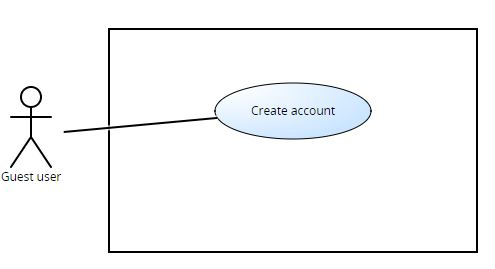
\includegraphics[width=\linewidth]{Guestuserusecase.jpg}
\caption{Guest user use case diagram}
\label{fig:UCD1}
\end{figure}
\subsubsection{Registered User}
\begin{figure}[H]
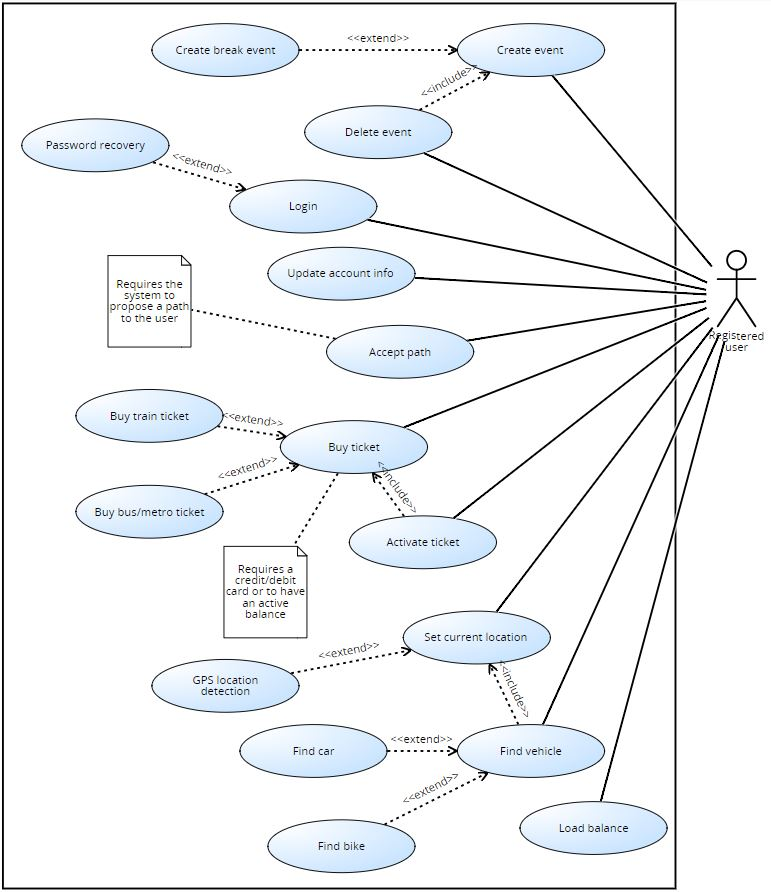
\includegraphics[width=\linewidth]{Registered_user_use_case.jpg}
\caption{Registered user use case diagram}
\label{fig:UCD2}
\end{figure}
\newpage
\subsection{Use Cases}
\paragraph{}
In the following section we include the use cases with their relative Sequence Diagrams and Statecharts.\\
\subsubsection{Create Account}
\begin{center}
\begin{tabular}{| p{3cm} || p{8cm} |}
\hline
Name & Create Account \\ \hline
Actors & Guest User \\ \hline
Assumptions & The user has started a registration form. \\ &The user has a valid e-mail address. \\ \hline
Flow Of Events & The user types his e-mail in the form. \\&The user reads the app's terms and conditions. \\& The user accepts the app's terms and conditions. \\& The user submits the information. \\& The system sends an e-mail to the user. \\& The user confirms the account through the link in the e-mail. \\ \hline
Exit Condition & The account is created \\ \hline
Exceptions & The e-mail is already linked to an account. The account is not created. \\
\hline
\end{tabular}
\end{center}
\begin{figure}[H]
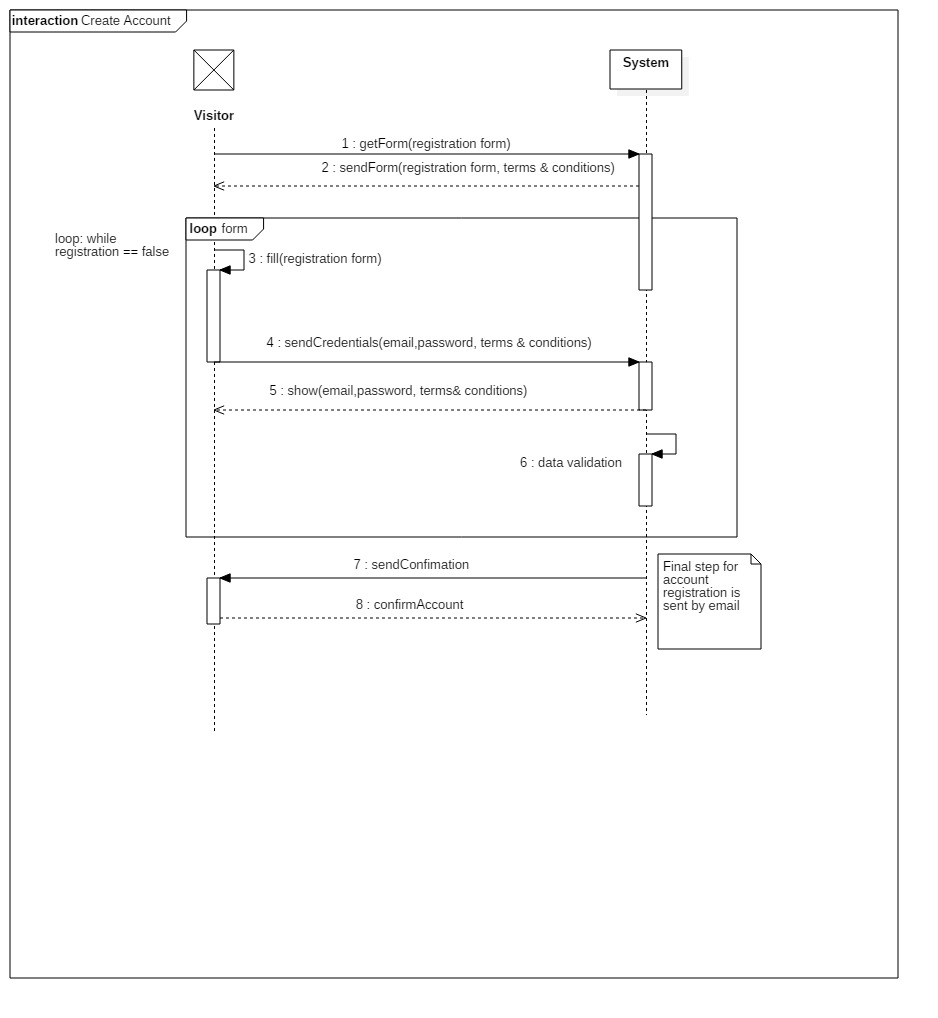
\includegraphics[width=\linewidth]{Create_Account.jpg}
\caption{Create Account Sequence Diagram}
\label{fig:SQ1}
\end{figure}
\subsubsection{Login}
\begin{center}
\begin{tabular}{| p{3cm} || p{8cm} |}
\hline
Name & Login\\ \hline
Actors & Registered User \\ \hline
Assumptions & The User has alreadty registered an account. \\&The user hasn't logged in yet. \\ \hline
Flow Of Events & The user has to open the app homepage. \\&The user has to input his information (e-mail and password). \\& The system checks if the information sent by the user are valid. \\ \hline
Exit Condition & The user is logged in the system \\ \hline
Exceptions & The information provided by the user are wrong.The user is not logged in. The page will refresh with an error message. \\
\hline
\end{tabular}
\end{center}
\begin{figure}[H]
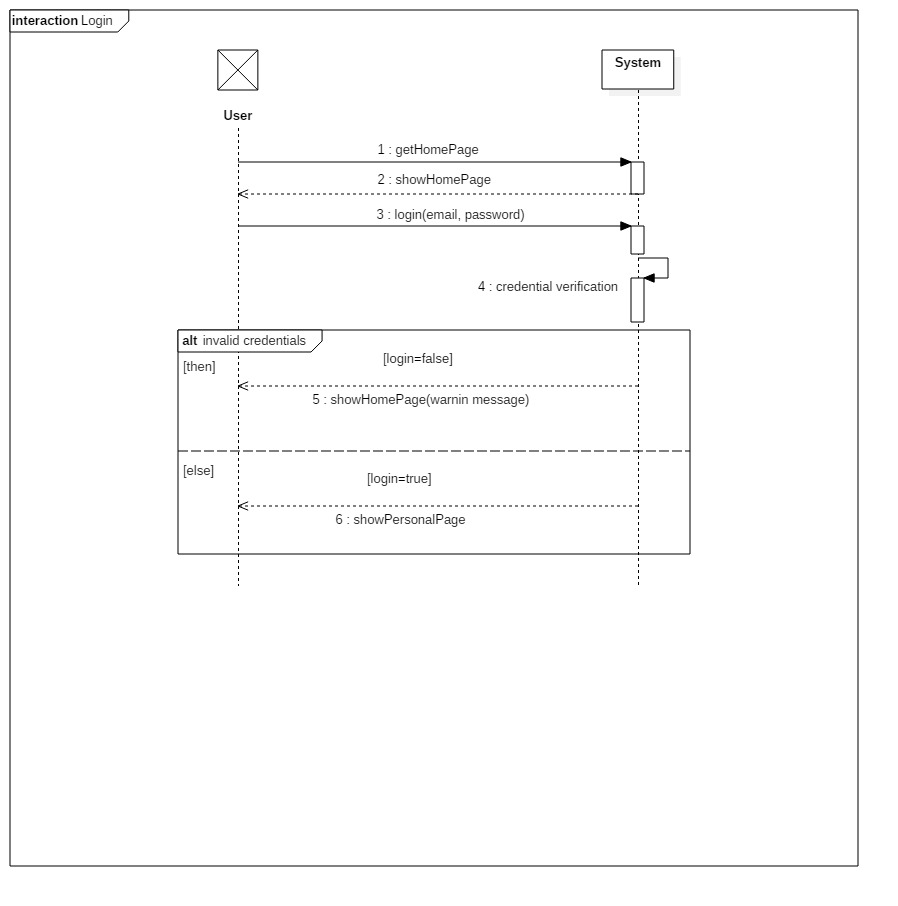
\includegraphics[width=\linewidth]{Login.jpg}
\caption{Login Sequence Diagram}
\label{fig:SQ2}
\end{figure}
\subsubsection{Create Event}
\begin{center}
\begin{tabular}{| p{3cm} || p{8cm} |}
\hline
Name & Create Event \\ \hline
Actors & Registered User \\ \hline
Assumptions & The user has already logged in the account. \\ \hline
Flow Of Events & The user has to go to the homepage of the app \\&The user has to open the "Create an event" page.\\&The user has to fill the information needed for the event (time, date, duration and location).\\&The user submits the information.\\&The system sends a confirmation request under the form of a review of the event.\\&The user confirms the information.\\&The system loads the information on the user's schedule. \\ \hline
Exit Condition & The event is successfully created and added on the schedule. \\ \hline
Exceptions &The user does not confirm the information. The system will go back to the information submission page and ask the user to input the correct information.\\& The connection is lost during the submission of the information. The event will not be created and the system will send an error message to the user who will be notified once the connection is restored. \\&The location does not exist on the map. The system will send an error message and the user will have to update the location. \\&The event is conflicting in time with another event, in this case the event will be created but the system will send the user a notification. \\
\hline
\end{tabular}
\end{center}
\begin{figure}[H]
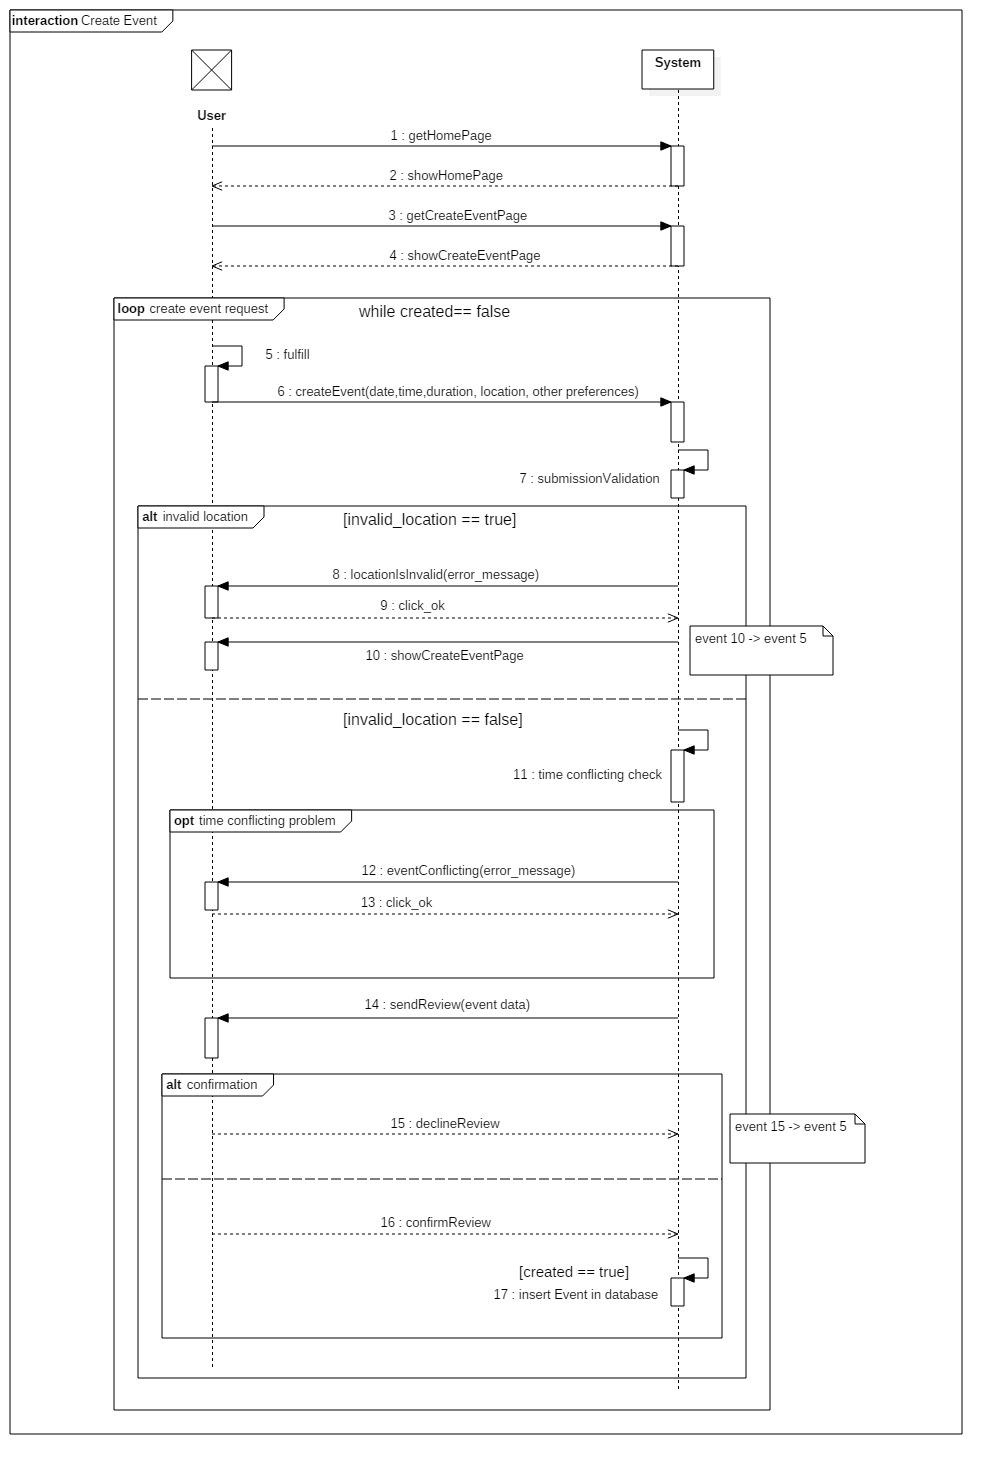
\includegraphics[width=\linewidth]{Create_Event.jpg}
\caption{Create Event Sequence Diagram}
\label{fig:SQ3}
\end{figure}
\subsubsection{Accept Path}
\begin{center}
\begin{tabular}{| p{3cm} || p{8cm} |}
\hline
Name &Accept Path \\ \hline
Actors & Registered User\\&Google Maps \\ \hline
Assumptions & The user is logged in the system.\\&The user has successfully created an event. \\ \hline
Flow Of Events & The system receives the new event\\&The system checks the preferences of the user.\\&The system will send the information of the event to Google Maps.\\&Google Maps will calculate a path.\\&Google Maps will send the path to the system.\\&The system will send the path to the user.\\&The user accepts the path.\\&The system verifies its compatibility in the users' schedule. \\ \hline
Exit Condition &The path is created. \\ \hline
Exceptions & The user doesn’t accept the path. The system will be notified and will have to start again by sending the information to Google Maps.\\&The system, after learning from Google Maps, realises there are incompatible events and send a warning to the user. The user will have to select which event is more important. The system will send the new information to Google Maps and start again.\\
\hline
\end{tabular}
\end{center}
\begin{figure}[H]
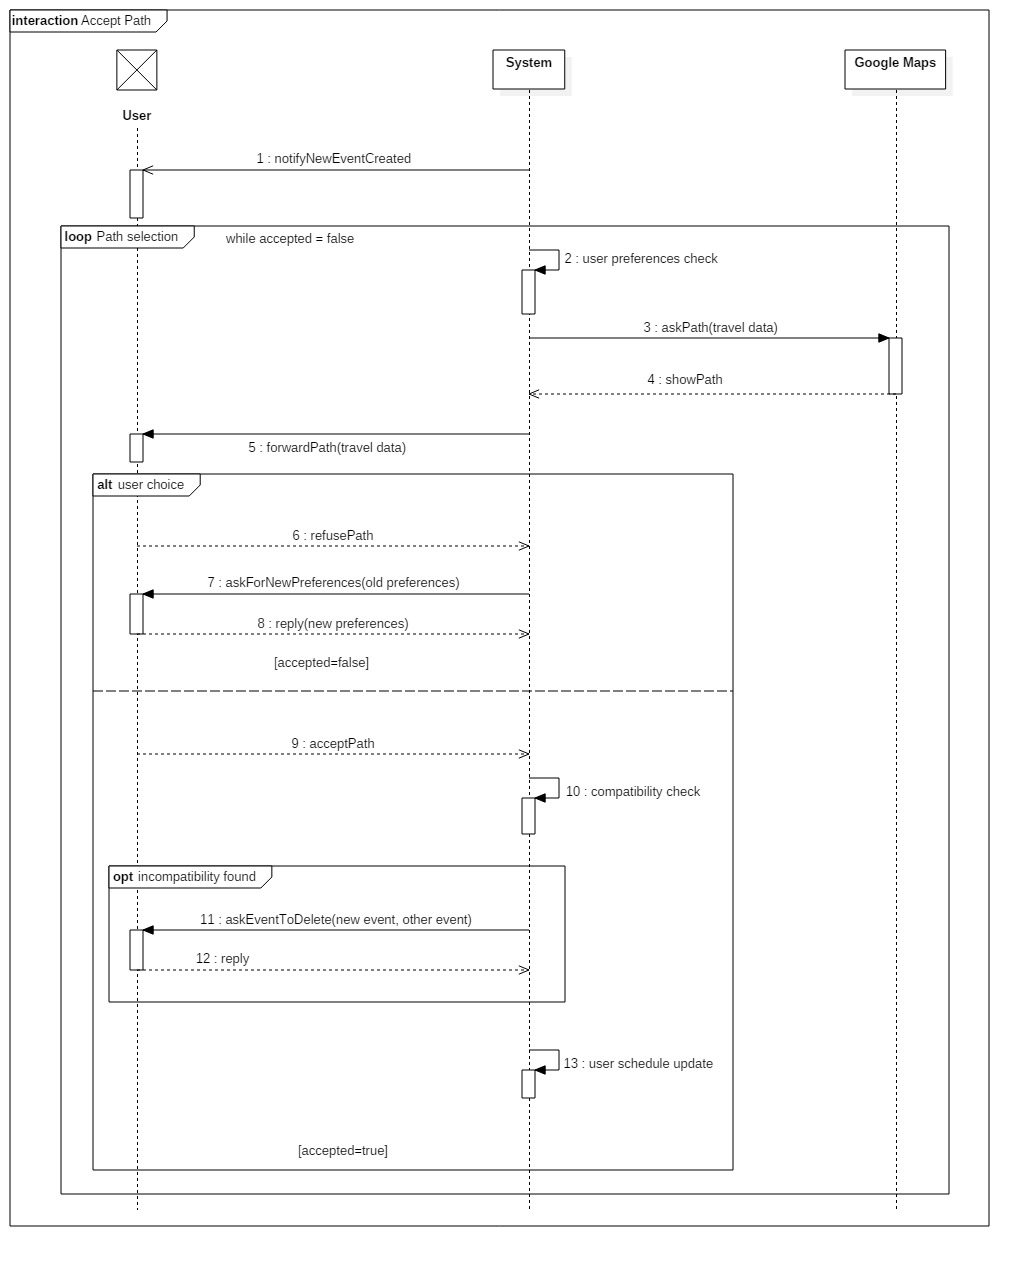
\includegraphics[width=\linewidth]{Accept_Path.jpg}
\caption{Accept Path Sequence Diagram}
\label{fig:SQ4}
\end{figure}
\subsubsection{Buy Ticket}
\begin{center}
\begin{tabular}{| p{3cm} || p{8cm} |}
\hline
Name & Buy Ticket \\ \hline
Actors & Registered User \\&Public Transportation System \\ \hline
Assumptions &The user is logged in the system.\\&The user has opened a balance in the app or has a credit/debit card connected to it. \\ \hline
Flow Of Events &The user clicks on “buy a ticket” from the homepage of the app.\\&
The user selects the ticket he wants to buy.\\&
The system receives the request and forwards it to the correct public transportation system.\\&
The public transportation system sends the information to Travlendar+’s system to complete the transaction.\\&
The system sends the information to the user.\\&
The user accepts the payment request.\\&
The user selects the payment option.\\&
The system sends the payment confirmation to the PTS.\\&
The PTS confirms the ticket.\\&
The PTS sends the ticket information to the system.\\&
The system saves the ticket in the user’s information. \\ \hline
Exit Condition &The ticket is available to be used by the user. \\ \hline
Exceptions &The balance does not have enough money to buy the ticket. The system will ask the user to select a different payment method.\\&
The credit card does not allow transaction. The system will ask the user to select a different payment method. \\&
The connection is lost between the system and the PTS. The system will have to ask to the user to start again from the selection of the ticket.
 \\
\hline
\end{tabular}
\end{center}
\begin{figure}[H]
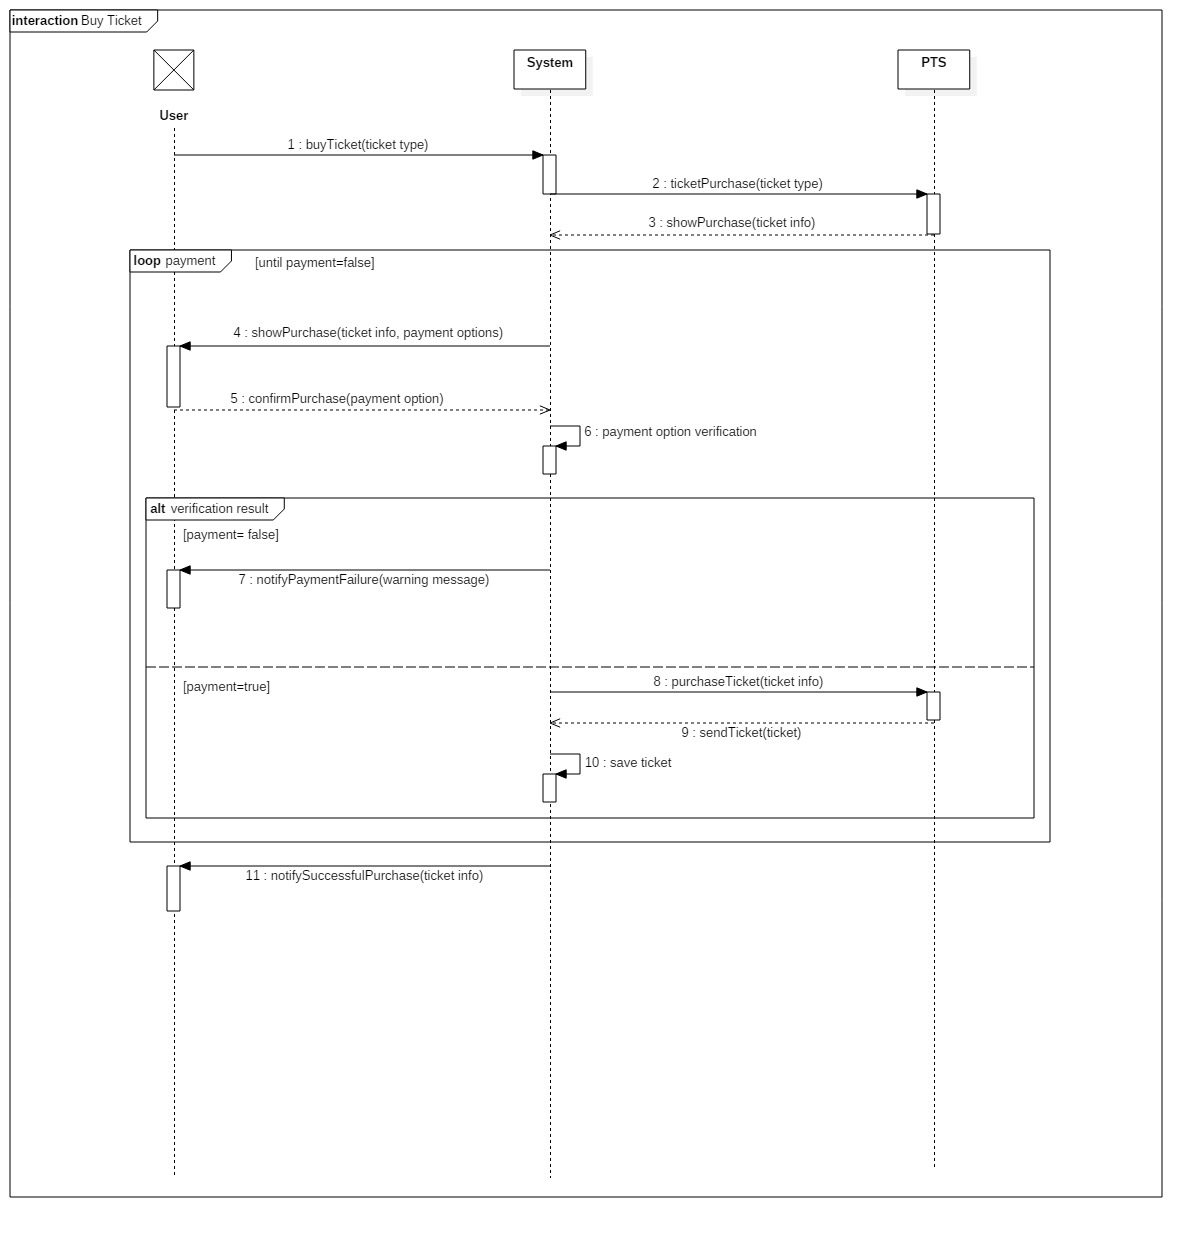
\includegraphics[width=\linewidth]{Buy_Ticket.jpg}
\caption{Buy Ticket Sequence Diagram}
\label{fig:SQ5}
\end{figure}
\subsubsection{Activate Ticket}
\begin{center}
\begin{tabular}{| p{3cm} || p{8cm} |}
\hline
Name &Activate Ticket \\ \hline
Actors &Registered user\\&
PTS
 \\ \hline
Assumptions &The user has logged in the system.\\&
The user has bought at least one ticket.\\&
The ticket has not been activated yet.
 \\ \hline
Flow Of Events &The user has to click on “My tickets” in his personal page.\\&
The system will send to the user the information about his ticket.\\&
The user will select the ticket that he wants to activate.\\&
The user will press on “Activate ticket”.\\&
The system will send a confirmation message to the user with a summary about the ticket.\\&
The user confirms the ticket.\\&
The system sends the details about the activation to the PTS.\\&
The PTS will send a confirmation of the activation of the ticket.
The system sends the confirmation to the user.\\&
The system will tag the ticket as “activated”.
 \\ \hline
Exit Condition &The ticket is activated and it becomes valid for the duration of the ticket.  \\ \hline
Exceptions & The user doesn’t confirm the ticket. The system will bring the user back to the selection of the ticket.\\&
There is a connection problem between the system and the PTS. The user will be notified of this and he will have to start the process again from the selection of the ticket.
\\
\hline
\end{tabular}
\end{center}
\begin{figure}[H]
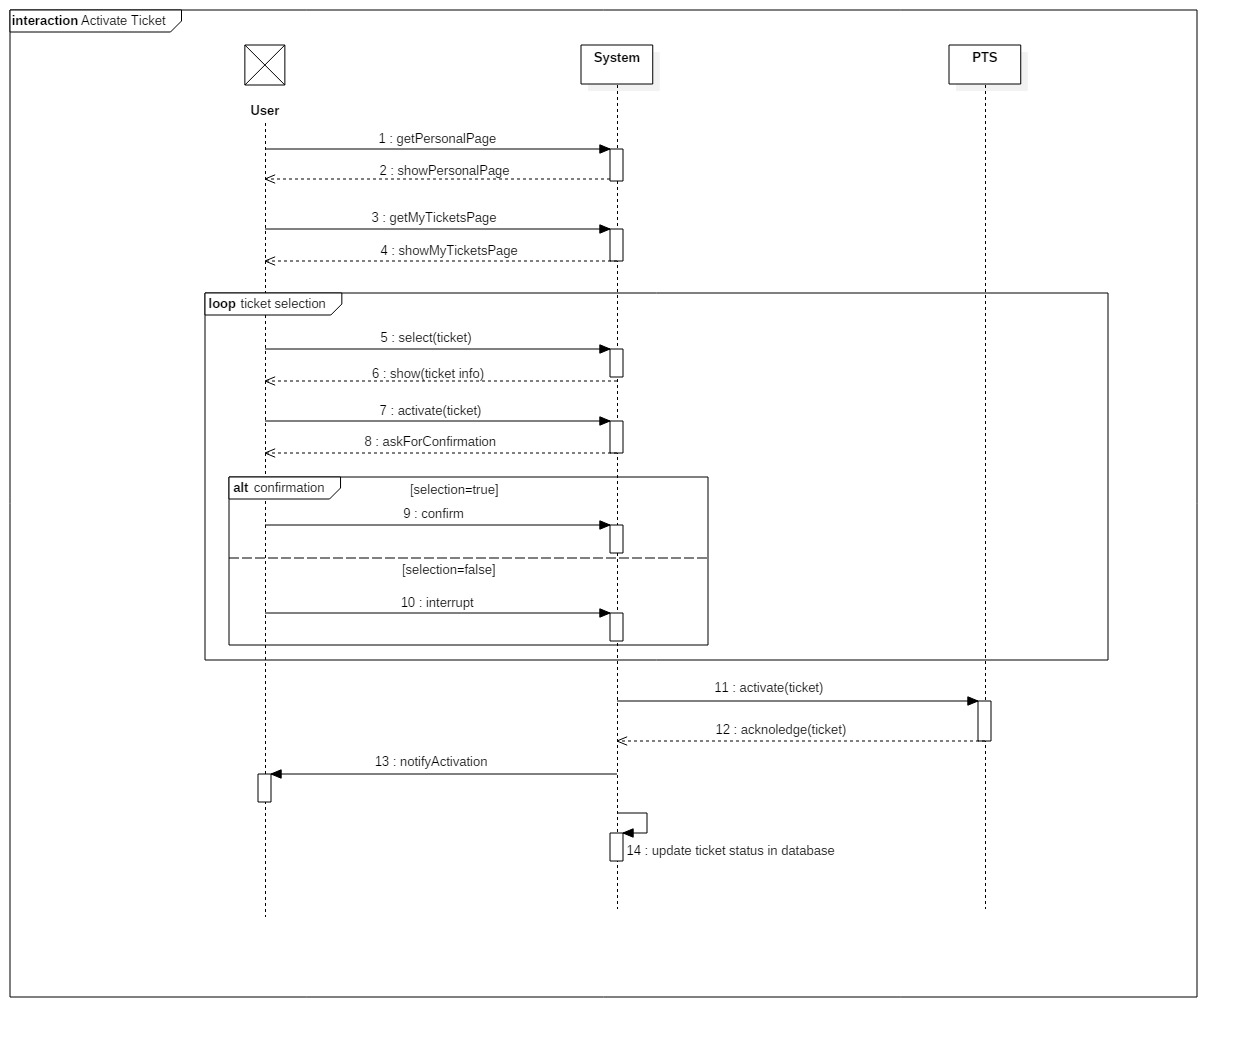
\includegraphics[width=\linewidth]{Activate_Ticket.jpg}
\caption{Activate Ticket Sequence Diagram}
\label{fig:SQ6}
\end{figure}
\subsubsection{Find Vehicle And Access Service}
\begin{center}
\begin{tabular}{| p{3cm} || p{8cm} |}
\hline
Name & Find Car/Bike And Access Service \\ \hline
Actors & Registered user\\&
Car-Sharing system (CSS) or Bike-Sharing system (BSS)
\\ \hline
Assumptions &The user is logged in the system.\\&
The user has a driving license.\\&
The information provided by the CSS are true.\\&
The user’s GPS is working and has the correct position.
 \\ \hline
Flow Of Events & The user has to click on “Find a vehicle” in the homepage of the app.\\&
The user has to select “Car” or “Bike”.\\&
The system sends a request for information to the CSS/ BSS.\\&
The CSS/ BSS sends the information needed to the system.\\&
The system will redirect the user to a map of his surroundings, with system.\\&
Once a vehicle is chosen, the system will redirect to that vehicle’s service app.
\\ \hline
Exit Condition & The user will be able to see available cars from different car sharing systems near his location and pick one. \\ \hline
Exceptions & There is a connection problem between the CSS(BSS) and Travlendar+’s system. The system will notify the user. The user will have to start again. \\
\hline
\end{tabular}
\end{center}
\begin{figure}[H]
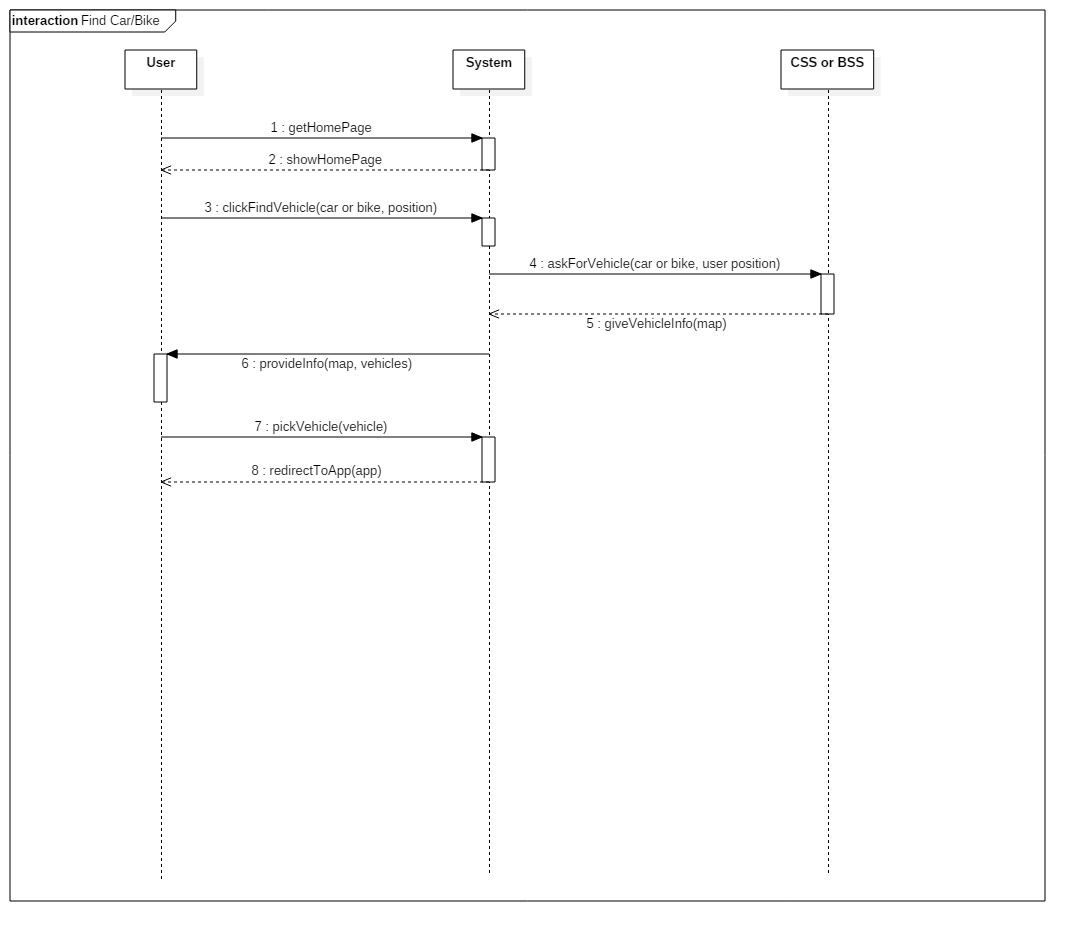
\includegraphics[width=\linewidth]{Find_Car_Bike.jpg}
\caption{Find Vehicle And Acceess Service Sequence Diagram}
\label{fig:SQ7}
\end{figure}
\subsubsection{Load Balance}
\begin{center}
\begin{tabular}{| p{3cm} || p{8cm} |}
\hline
Name &Load Balance \\ \hline
Actors &Registered User\\&
Bank \\ \hline
Assumptions & The user has a credit/debit card connected to the account or
The user has bought a code to load the balance from a certified shop.\\ \hline
Flow Of Events &The user has to click on “Load balance”.\\&
The system will redirect him to the loading balance page.\\&
The user will have to select “Credit/debit Card” or “Use a code”.\\&
\begin{enumerate}
\item Credit/Debit Card case: The user has to select the amount of money he wishes to load into the balance.
The system sends the request to the bank.
The bank confirms the transaction.
\item Use a code:
The system asks the user to insert the code written on the card he bought.
The user inserts the information requested and confirms.
The system checks that the information is correct.
 \end{enumerate}\\& The system sends a confirmation message to the user. \\ \hline
Exit Condition & The balance is updated. \\ \hline
Exceptions & The bank does not allow the transaction. The system requests the user to try again.\\&
The information sent by the user are incorrect. The system asks the user to check if the code is correct and to try again.
\\
\hline
\end{tabular}
\end{center}
\begin{figure}[H]
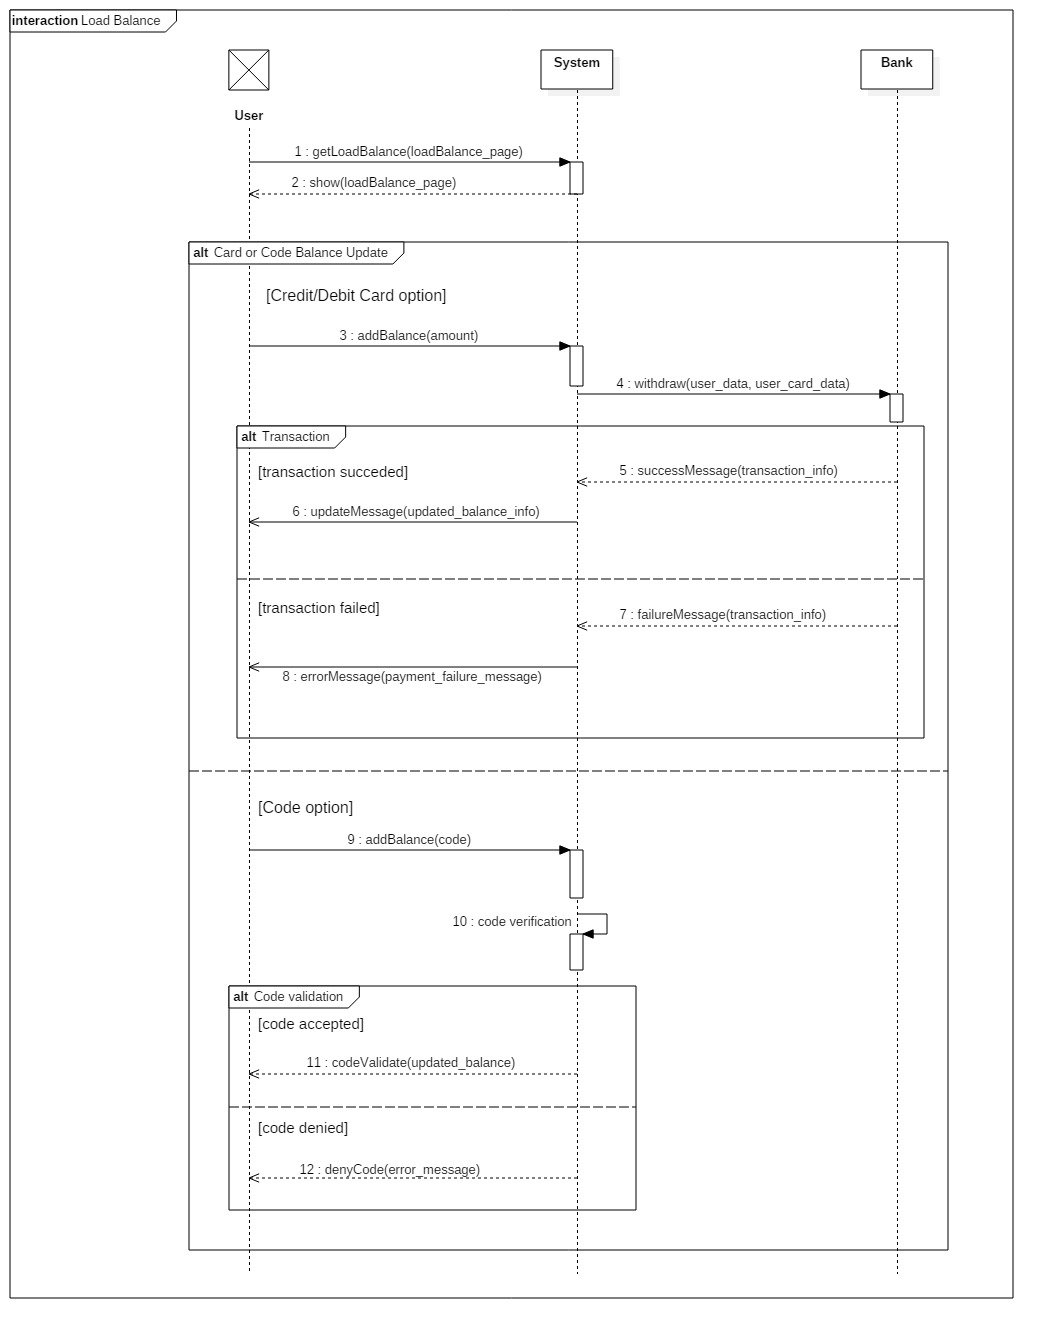
\includegraphics[width=\linewidth]{Load_Balance.jpg}
\caption{Load Balance Sequence Diagram}
\label{fig:SQ8}
\end{figure}

\newpage
\section{Formal Analysis Using Alloy}
\subsection{Model Representation}
\paragraph{}
This Alloy document generates a model of the system in a precise moment. It represents a “photography” of the system and deals more with its global coherence than with the integrity of the transitions. In short, the most important properties of the model are:
\begin{itemize}
\item{} Users and external actors belong to the same system (Travlendar+).
\item{} The users are distinguished in guest and registered users. Since only the registered ones can operate on the system, we are referring to them saying "users".
\item{} Every user can define some settings and the system must not violate them when it suggests some paths.
\item{} Every user owns a schedule containing every event they need to attend.
\item{} The system suggests some paths for the users' events, and those paths are grouped in the users' daily paths.
\item{} The system can suggest an alternative path for an event only if the main path has been refused or it is not "in time".
\item{} The external actors determine the presence of their transports as options in t he system and (some of the actors) the possiblity to buy tickets for those transports.
\end{itemize}
\paragraph{Alloy Code\\} The following is the source code of our alloy model.
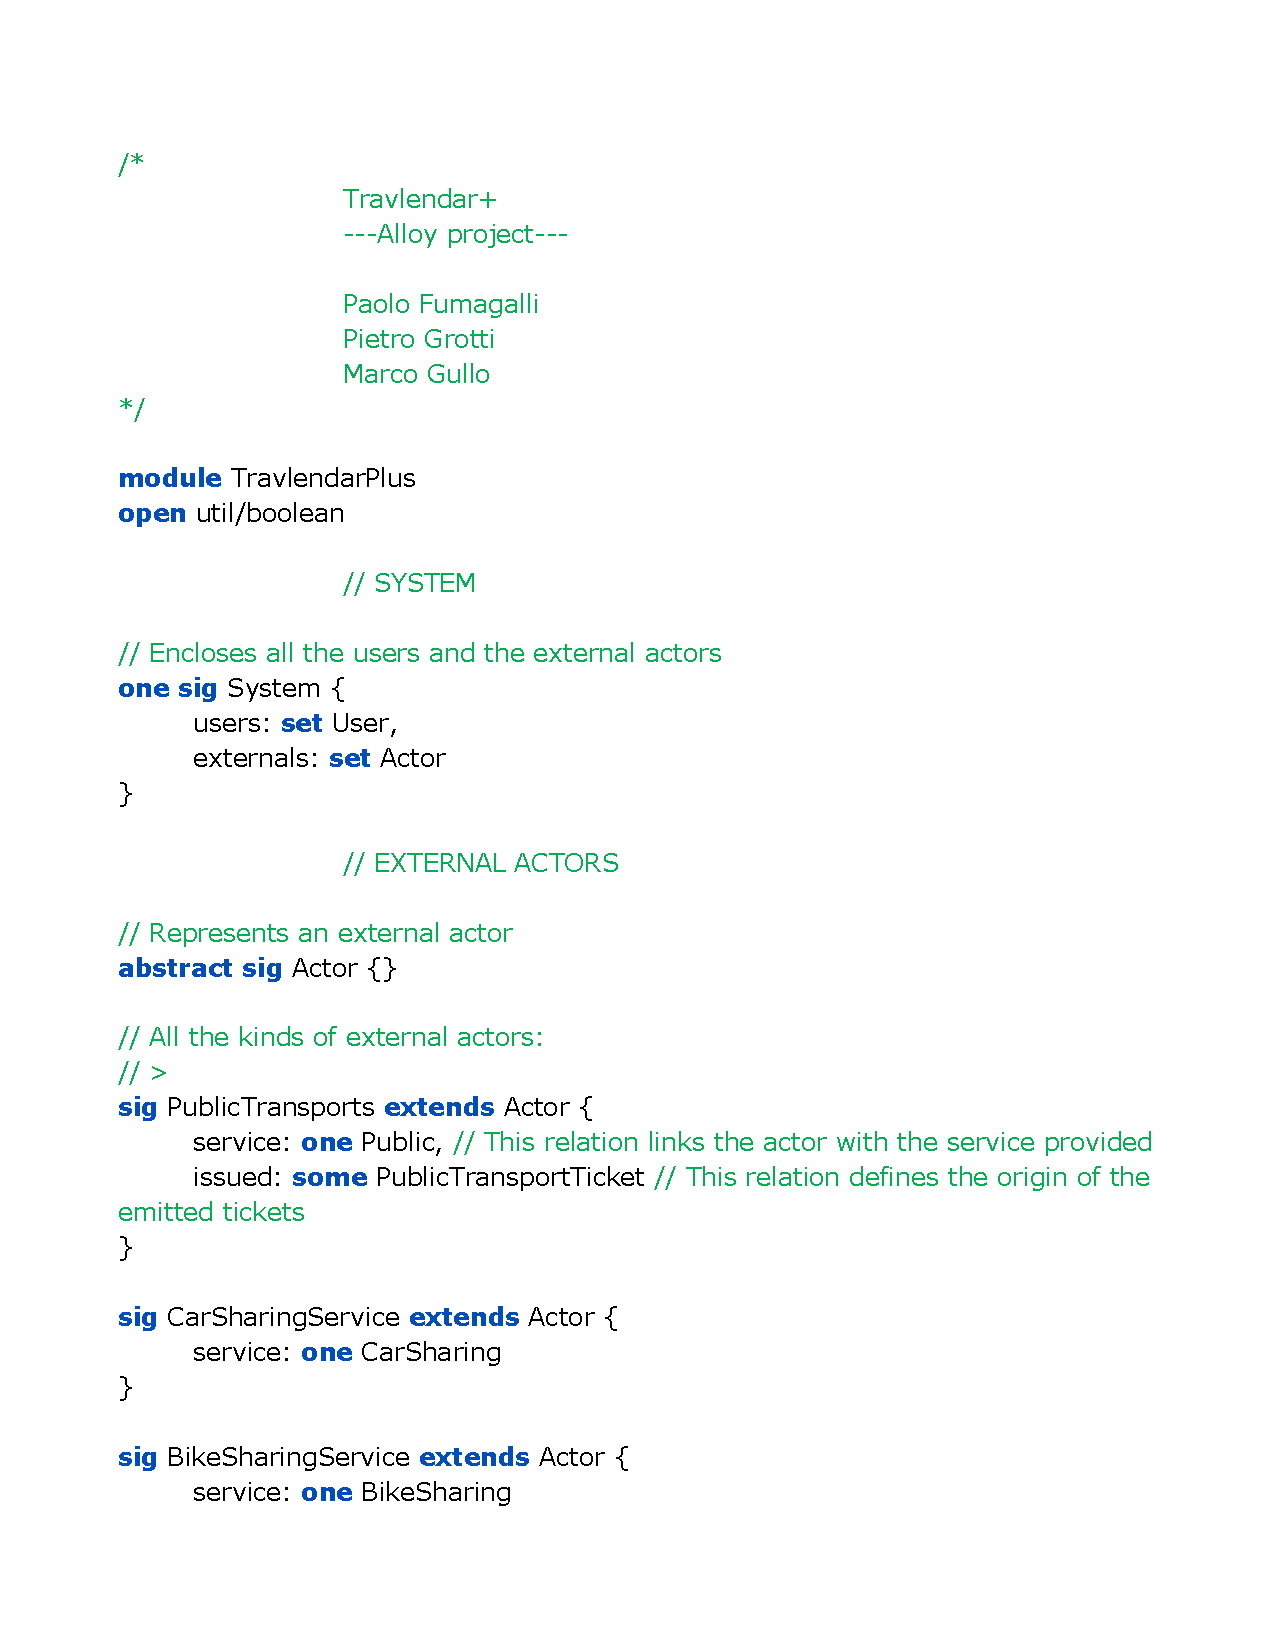
\includepdf[pages=-,pagecommand={}, width=\textwidth]{Alloy_text.pdf}
\subsection{Instances}
\subsubsection{Instance 1}
\begin{figure}[H]
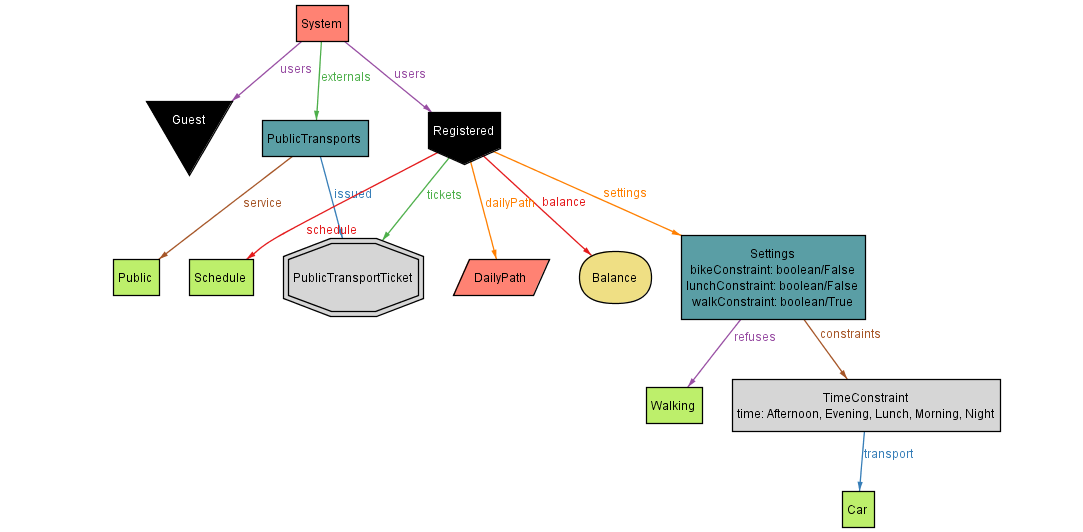
\includegraphics[width=\linewidth]{Instance_1.png}
\caption{First Instance}
\label{fig:ALLOY1}
\end{figure}
\paragraph{Instance 1\\}
In this instance there are no users’ events, so the system doesn’t generate any suggested path. However, there exist users’ settings, schedules, daily paths and system’s external actors. The system is ready to add an event in the registered user’s schedule. 
\subsubsection{Instance 2}
\begin{figure}[H]
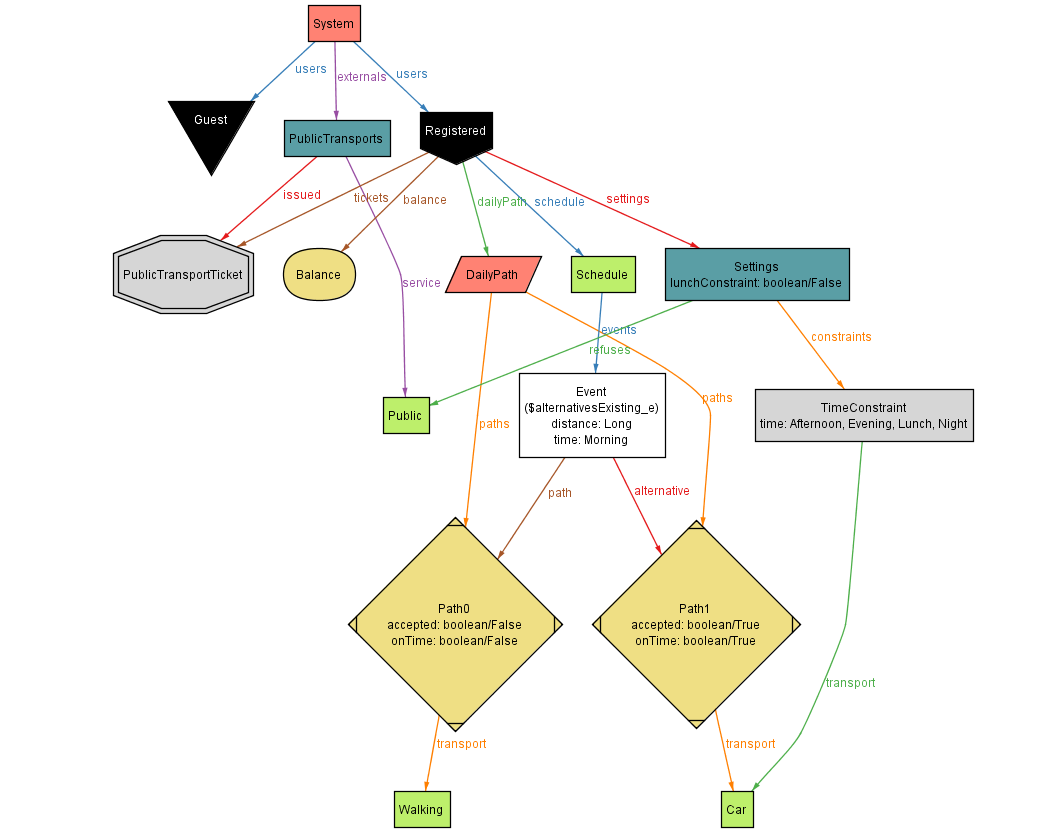
\includegraphics[width=\linewidth]{Instance_2.png}
\caption{Second Instance}
\label{fig:ALLOY2}
\end{figure}
\paragraph{Instance 2\\}
In this instance, the registered user has one event in his schedule. The system suggests a main path for this event, but it is neither “in time” or “accepted by the user”. So, the system suggests an alternative path for the same event, which allows the user to be in time.
\subsubsection{Instance 3}
\begin{figure}[H]
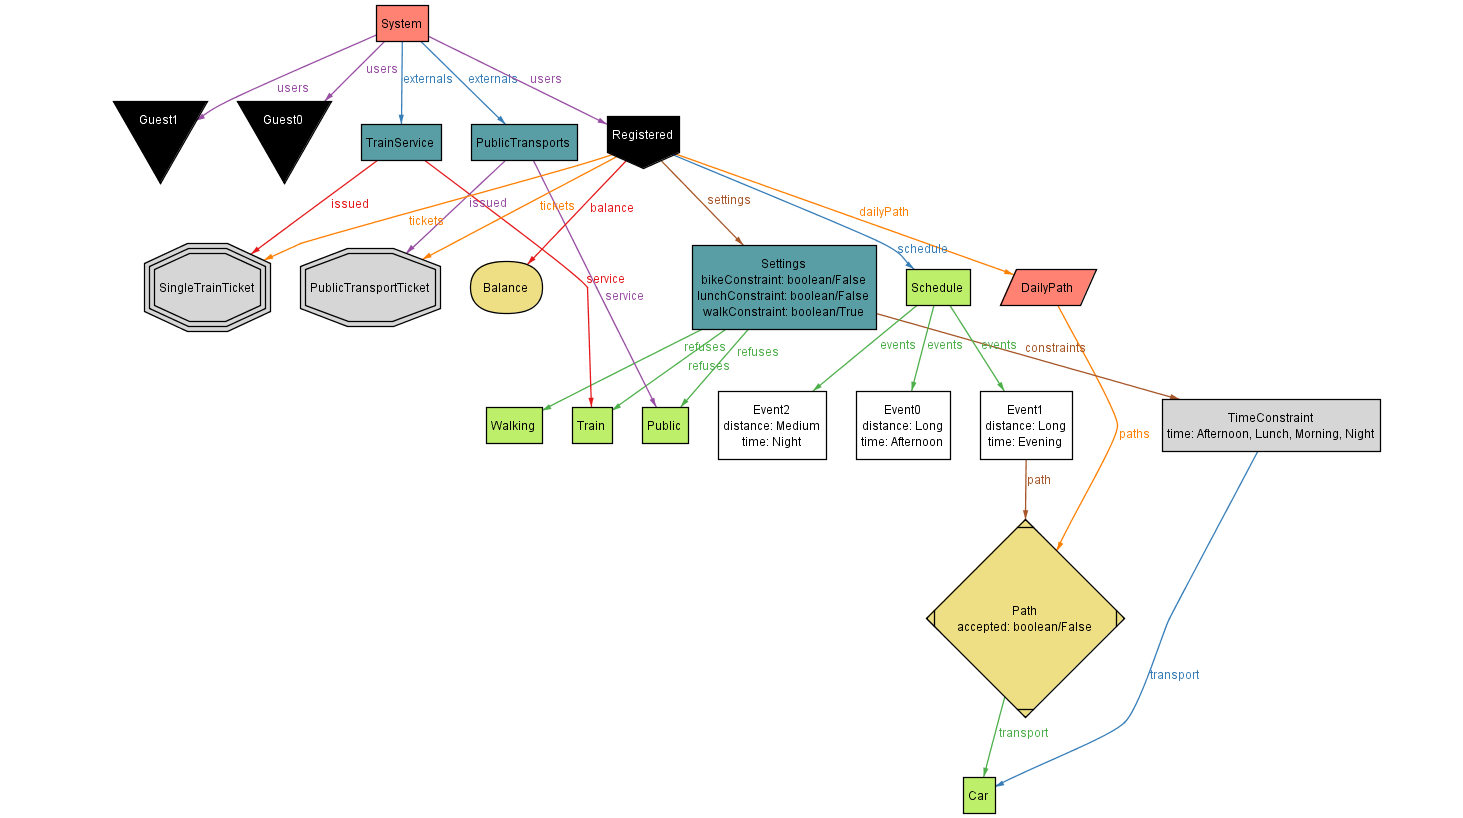
\includegraphics[width=\linewidth]{Instance_3.png}
\caption{Third Instance}
\label{fig:ALLOY3}
\end{figure}
\paragraph{Instance 3}
In this instance, both Public Transports and Train Service exist as external actors in the system. The registered user owns in his account a single train ticket and a public transports ticket. The link between the tickets and the actors which allowed their purchase is highlighted by the relation “issued”.
\newpage
\section{Effort Spent}
\begin{itemize}
\item{Fumagalli Paolo:} 25 hours.
\item{Grotti Pietro:} 25 hours.
\item{Gullo Marco:} 25 hours.
\end{itemize}
\section{References}
\subsection{Tools Used}
\begin{itemize}
\item{} Google Doc
\item{} Signavio
\item{} Alloy Analyzer 4.2
\item{} StarUML 5.3
\item{} TeXworks
\end{itemize}
\end{document}